% !TeX spellcheck = cs_CZ
% Musilova2009MA1

\begin{example}\label{mai:exam011}
  Zjistěte ortogonální doplněk \(\langle(1,-3,2),(2,1,5)\rangle\bot^.\). (Zdroj:
  \cite[s.~3]{MosnaMA3})
  \newline\textbf{Řešení}:
  Hledáme vektor \((x, y, z)\), jehož skalární součin je se zadanými vektory roven nule. Budeme 
  tedy řešit (úpravou na Gaussův tvar pomocí elementárních úprav) homogenní soustavu rovnic
  zadanou maticí
  \begin{equation*}
     \left(
       \begin{array}{ccc|c}
          1  &  -3  & 2 & 0 \\
          2  &   1  & 5 & 0
       \end{array}
     \right)\sim
     \left(
       \begin{array}{ccc|c}
          1  &  -3  & 2 & 0 \\
          0  &   7  & 1 & 0
       \end{array}
     \right)\
  \end{equation*}
  Odtud dostáváme \(z = \alpha\), \(7y + z = 0\) \(\Rightarrow\) \(y = -\frac{1}{7}\alpha\), \(x
  +\frac{3}{7}\alpha + 2\alpha = 0\) \(\Rightarrow\) \(x = -\frac{17}{7}\) neboli 
  \begin{equation*}
  (x, y, z) =\alpha\left(-\frac{17}{7}, -\frac{1}{7}, 1\right) = \alpha(17, 1, -7)
  \end{equation*}

  V dalších příkladech budeme nuly na pravé straně soustavy vynechávat a upravovat na
  výhodnější tvar
  \begin{equation*}
       \begin{pmatrix}
          1  &  -3  & 2  \\
          2  &   1  & 5
       \end{pmatrix}
       \sim
       \begin{pmatrix}
          1  &  -3  & 2 \\
          0  &   7  & 1
       \end{pmatrix}
       \sim
       \begin{pmatrix}
          1  &   0  & \frac{17}{7}  \\
          0  &   7  & 1
       \end{pmatrix}
       \sim
       \begin{pmatrix}
          7  &   0  & 17 \\
          0  &   7  & 1
       \end{pmatrix}.
  \end{equation*}
  Odtud již snadno zjistíme, že vektor \((x, 1, -7)\) jistě vyhovuje druhé rovnici. Dosadíme-li ho 
  do první rovnice, dostaneme \(7x + 17\cdot(-7) = 0\) a \(x = 17\).

  Hledaný ortogonální doplněk je tedy lineární obal $$\langle(17, 1, -7)\rangle^\bot.$$
  
    {\centering
     \captionsetup{type=figure}
    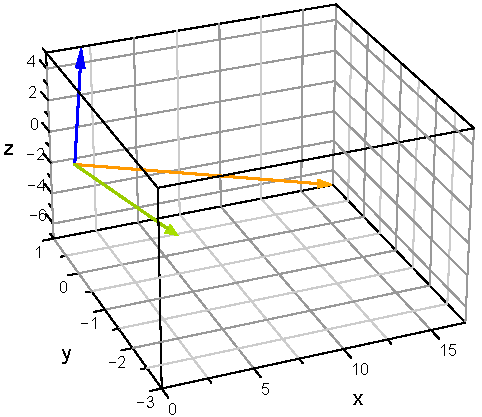
\includegraphics[width=0.5\linewidth]{mai_fig025.pdf}
    \captionof{figure}[Ortogonální doplněk]{Vizualizace vektorového prostoru a jeho    
             ortogonálního doplňku pomocí sw MatLab - MuPAD příkazem:\newline
             \texttt{plot(plot::Arrow3d([1,-3,2]), plot::Arrow3d([2,1,5]), 
             plot::Arrow3d([17,1,-7]))}}
    \label{LA:fig_ort01}
    \par}
\end{example}
